\documentclass[onecolumn, draftclsnofoot,10pt, compsoc]{IEEEtran}
\usepackage{graphicx}
\usepackage{url}
\usepackage[utf8]{inputenc}
\usepackage{setspace}
\usepackage{caption}
\usepackage[nonumberlist,acronym]{glossaries}
\usepackage{hyperref}
\usepackage{nomencl}
\usepackage{geometry}
\usepackage{color}
\usepackage{float}

%\usepackage[justification=centering]{caption}

\graphicspath{ {images/} }
\geometry{textheight=9.5in, textwidth=7in}

\definecolor{codegreen}{rgb}{0,0.6,0}
\definecolor{codegray}{rgb}{0.5,0.5,0.5}
\definecolor{codepurple}{rgb}{0.58,0,0.82}
\definecolor{backcolour}{rgb}{1.0,1.0,1.0}

\usepackage{listings}
\lstset{
         basicstyle=\footnotesize\ttfamily,
         backgroundcolor=\color{backcolour},
    	 commentstyle=\color{codegreen},
    	 keywordstyle=\color{magenta},
    	 numberstyle=\tiny\color{codegray},
    	 stringstyle=\color{codepurple},
         morecomment=[l][\color{magenta}]{\#},
         numberstyle=\tiny,
         numbersep=5pt,
         numbers=left,
         tabsize=1,                
         extendedchars=true,      
         breaklines=true,        
         showspaces=false,      
         showtabs=false,       
         xleftmargin=17pt,
         framexleftmargin=17pt,
         framexrightmargin=5pt,
         framexbottommargin=4pt,
         showstringspaces=false 
 }

\def \CapstoneTeamNumber{55}
\def \GroupMemberOne{Riley Rimer}
\def \GroupMemberTwo{River Hendriksen}
\def \GroupMemberThree{Corey Hemphill}
\def \CapstoneProjectName{CoverageJSON Response Handler for OPeNDAP}
\def \CapstoneSponsorCompany{NASA Jet Propulsion Laboratory}
\def \CapstoneSponsorPerson{Lewis John McGibbney}

\def \DocType{	%Problem Statement
				%Requirements Document
				%Technology Review
				Design Document
				%Progress Report
				}
			
\newcommand{\NameSigPair}[1]{\par
\makebox[2.75in][r]{#1} \hfil 	\makebox[3.25in]{\makebox[2.25in]{\hrulefill} \hfill		\makebox[.75in]{\hrulefill}}
\par\vspace{-12pt} \textit{\tiny\noindent
\makebox[2.75in]{} \hfil	\makebox[3.25in]{\makebox[2.25in][r]{Signature} \hfill	\makebox[.75in][r]{Date}}}}
% 3. If the document is not to be signed, uncomment the RENEWcommand below
\renewcommand{\NameSigPair}[1]{#1}
%%%%%%%%%%%%%%%%%%%%%%%%%%%%%%%%%%%%%%%
\newglossarystyle{mylong}{%
  \setglossarystyle{long}%
  \renewenvironment{theglossary}%
     {\begin{longtable}[l]{@{}p{\dimexpr 2cm-\tabcolsep}p{0.8\hsize}}}% <-- change the value here
     {\end{longtable}}%
 }

\makenomenclature
\makeglossaries
\newglossaryentry{OPeNDAP}
{
    name=OPeNDAP,
    description={Open-source Project for a Network Data Access Protocol. An HTTP protocol/architecture that 	transfers data from a source to a client}
}
\newglossaryentry{Client}
{
    name=Client,
    description={Within the scope of networking a client is the end user that will be asking the server for 	information}
}
\newglossaryentry{Server}
{
    name=server,
    description={A called upon system requested by a client, generally over a network}
}
\newglossaryentry{NASA JPL}
{
    name=NASA JPL,
    description={National Aeronautics and Space Administration Jet Propulsion Laboratory}
}
\newglossaryentry{CoverageJSON}
{
    name=CovJSON,
    description={An extension of the JSON (JavaScript Object Notation) language made to transmit geotemporal data. JSON is one a few 	 standard means by which data is transmitted through networks. It is notable for being human readable, therefore easier to parse 	 and manage}
}
\newglossaryentry{HTTPS}
{
    name=HTTPS,
    description={Hypertext Transfer Protocol Secure. A means of secure communication over a computer network}
}
\newglossaryentry{Hyrax}
{
    name=Hyrax,
    description={A data server that receives requests via OPeNDAP. Hyrax is mainly used for the gathering and processing data then 	   returning it to the client}
}
\newglossaryentry{Front-end}
{
    name=OLFS,
    description={Front end, in Java, for the Hyrax data server}
}
\newglossaryentry{back-end}
{
    name=BES,
    description={back end, in C++, for the Hyrax data server}
}
\newglossaryentry{GET}
{
    name=GET,
    description={A request from a client to a server to receive data that the server has}
}
\newglossaryentry{POST}
{
    name=POST,
    description={A request from a client to a server to modify/recieve data that the server has}
}
\newglossaryentry{CppUnit}
{
    name=CppUnit,
    description={A unit testing framework that is available for c++.}
}
\newglossaryentry{Coverage}
{
    name=Coverage,
    description={A digital representation of a spatio-temporal domain.}
}
\newacronym{FEA}{FEA}{Finite Element Analysis}
\renewcommand{\glossarysection}[2][]{}
%%%%%%%%%%%%%%%%%%%%%%%%%%%%%%%%%%%%%%%
\begin{document}
\begin{titlepage}
    \pagenumbering{gobble}
    \begin{singlespace}
        \hfill    
        \par\vspace{.2in}
        \centering
        \scshape{
            \huge CS Capstone \DocType \par
            {\large\today}\par
            \vspace{.5in}
            \textbf{\Huge\CapstoneProjectName}\par
                        \vspace{.5in}

            \vfill
            {\large Prepared for}\par
            \Huge \CapstoneSponsorCompany\par
            \vspace{5pt}
            {\Large\NameSigPair{\CapstoneSponsorPerson}\par}
            {\large Prepared by }\par
            Group\CapstoneTeamNumber\par
            \vspace{5pt}
            {\Large
                \NameSigPair{\GroupMemberOne}\par
                \NameSigPair{\GroupMemberTwo}\par
                \NameSigPair{\GroupMemberThree}\par
            }
            \vspace{20pt}
        }
        \begin{abstract}
        	ABSTRACT 
        \end{abstract}     
    \end{singlespace}
\end{titlepage}
\newpage
\pagenumbering{arabic}
\tableofcontents
% 7. uncomment this (if applicable). Consider adding a page break.
%\listoffigures
%\listoftables
\clearpage
%start doc sections
\section{Overview}
\subsection{Purpose} 
The purpose of this document is to describe the initial design plans that will be used to develop a \gls{CoverageJSON} Data Response Handler for the OPeNDAP project. This document will cover the following sections from different viewpoints:
\begin{itemize}
\item The host architecture that will be used for \gls{HTTPS} Network Handling and managing client requests. 
\item OPeNDAP, the protocol that the response handler will be implemented for.
\item The CoverageJSON scientific coverage data format.
\item The testing framework that will be used to ensure the reliability of the code we create.
\item The web application framework that will be used.
\end{itemize}

\subsection{Project Scope}
This document will provide information on the design of components that are to be implemented in the finished response handler. The purpose of this project is to integrate a new response handler for the CoverageJSON data format into the currently existing collection of data response handlers within the OPeNDAP network data access protocol. Implementing this will involve interfacing with the OPeNDAP team as well as NASA Jet Propulsion Laboratory (JPL) to gather requirements and acquire a general understanding of the OPeNDAP code base. OPeNDAP does not currently provide a handler for a coverage data format like CoverageJSON, which is a structure that associates positions in space and time with the corresponding data values. The addition of the CoverageJSON format into OPeNDAP will allow for more fluid development of coverage data based web applications by NASA JPL and all other OPeNDAP users. Due to the desire for the new CoverageJSON response handler to be integrated into the OPeNDAP open-source project, the data handler will need to be accompanied by extensive documentation and testing. This project will also include testing current NASA satellite data in OPeNDAP on the proposed response handler and creating a promotional poster for the American Geophysical Union.

\subsection{Intended Audience}
This document is intended primarily for developers of the \gls{OPeNDAP} protocol. However, this document may also be useful for \gls{NASA JPL}, and other developers that intend to contribute to or implement the OPeNDAP protocol within their data server systems. From an OPeNDAP perspective, this document will act as a confirmation that their requirements are being met. For others, it will serve as a high-level view of how we plan to approach the design and implementation of the CovJSON response handler for OPeNDAP. This document may represent requirements that differ from the requirements that the client explicitly requested; if so, they may have been deemed necessary by the developers for the creation of the project. This document has not yet been reviewed by the client and will be revised at a future date.

\section{Design Description}

\subsection{Design Stakeholders}
The design stakeholders of this project include both the users and the developers of OPeNDAP, Hyrax, and CovJSON. This includes Lewis John McGibbney and NASA JPL, as well as James Gallagher of OPeNDAP. The completion of the implementation of this design will help further accommodate web development on coverages, and extend the usability of the CoverageJSON format. OPeNDAP is also a stakeholder due to the intended incorporation of this project into OPeNDAP.

\subsection{Design Rationale}
The design for this project is heavily influenced by the fact that almost all of the work in the project is on systems that were already implemented. This leads the design to take heavy cues from the existing system implementations to avoid conflicting design and to remain consistent with the development standards of the project. This is most prevalent in the coding itself that will take place in OPeNDAP, where this project's implementation will need to align strictly to the current code base for OPeNDAP so it smoothly transitions into the OPeNDAP project upon completion. Due to the scope of the systems being worked on there is also a lot of information relevant to the design for this project that has not been discussed yet, which is why parts of the current design are rather shallow. This document will be periodically updated as more of the design planning is worked out with the current members of OPeNDAP, due to their integral nature in the final implementation of this project.

For the reasons discussed the writers of this document have decided to forgo some standards of the IEEE design documentation because they do not apply to the work that will come from this design. As such viewpoints have been removed in favor of components, as those are the parts of the design that must be considered for this project to be successful. To not completely remove the standards set in place the document still discusses the viewpoints for each component, this is so the developers can consider the constraints relegated to those views. 

%%%%%%%%%%%%%%%%%%%%%%%%%%%%%%%%%%%%%%%
\section{Components}

\subsection{Component: Host Architecture}
\subsubsection{Purpose}
The purpose of having a dedicated host architecture is twofold. One, it allows for developers of this project to follow a standard that is already implemented by the architecture. And two it saves time in integration into OPeNDAP which already uses this host architecture. Having an HTTPS handler already in place is imperative for the creation and testing of a response handler. 
\subsubsection{Viewpoint}
The view point for this component is logical since it is a system that is already in place and the development of the CovJSON handler will use libraries and methods already created in the \gls{Hyrax} data server \cite{IEEE}. Besides the back-end conversion from the NASA JPL scientific data format to the CovJSON standard, all calls and functions to any networking system will be done with methods from the Hyrax data server.
\subsubsection{Concerns}
There are minor concerns with integration into the Hyrax data server. One limit is time, and the ability for the developers on this project to fully understand a complicated system like Hyrax within a limited time set may be an issue. However, the developers have resources for Hyrax such as employees and founders that may make this problem a non-issue. 
\subsubsection{Functionality}
Hyrax's main purpose is broken into two parts, the \gls{Front-end} (OLFS) and the \gls{back-end} (BES). Functionally the Hyrax data server is a means for data to be requested by a client from a server using OPeNDAP protocols \cite{Hyrax}. The design of this project is entirely based around the use of OPeNDAP and thus must be based on the Hyrax implementation. \autoref{fig:clientserver} shows how the clients system interacts with the Server \cite{clientserver}.
\begin{figure}[H]
    \centering
    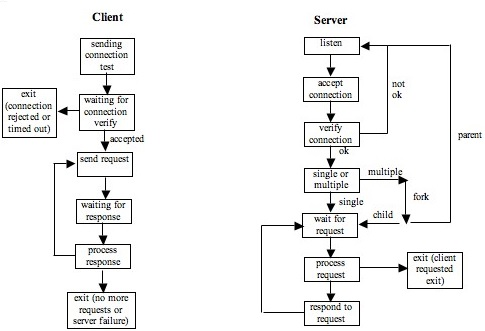
\includegraphics[width=4in,scale=1.0]{Hyrax_state_diagram.jpg}
    \caption{Client Server relationship Hyrax}
    \label{fig:clientserver}
\end{figure}

\begin{figure}[H]
    \centering
    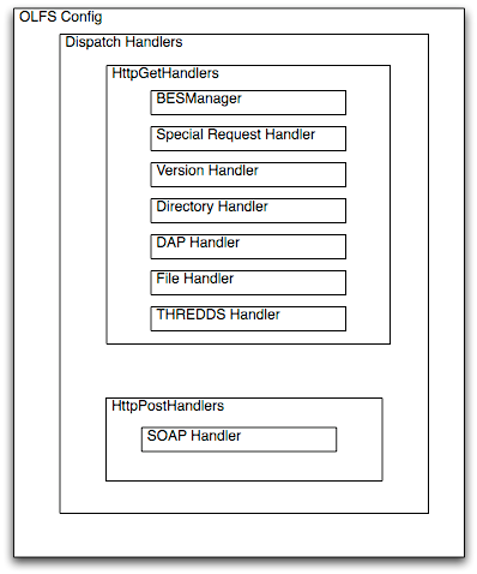
\includegraphics[width=3in,scale=1.0]{handler.png}
    \caption{OLFS Handler}
    \label{fig:handlerolfs}
\end{figure}
\subsubsection{OLFS}
The OLFS works as a receiver for requests from clients, authenticating requests and ensuring DAP2 compliance. OLFS is implemented in the Java programming language, which contrasts with the BES which is primarily implemented in C++. The BES is the prime target for this project, however understanding and setting up the OLFS is a must to effectively implement and test the CovJSON response handler. \\
\autoref{fig:handlerolfs} shows the dispatch handler for the Hyrax server. The dispatch is an ordered list that specifies what BES calls must be made to handle an incoming request. This list is broken into \gls{GET} and \gls{POST} HTTPS requests and configuration for response handlers can be applied for both.\autoref{fig:OLFS} represents a basic implementation of the Hyrax OLFS.
Going through the code quickly it can be seen that BESMANAGER sets the configurations for BES. While the dispatch handler goes through both the GET and POST requests as mentioned before, the OLFS will send BES commands to the BES which will then run conversion commands and return the data to the OLFS again which will then return it to the client. The project's engineers will have to know how to initially set up the Hyrax front-end and send the correct BES commands to run CovJSON request handler. \cite{OLFS}
\begin{figure}[H]
    \centering
    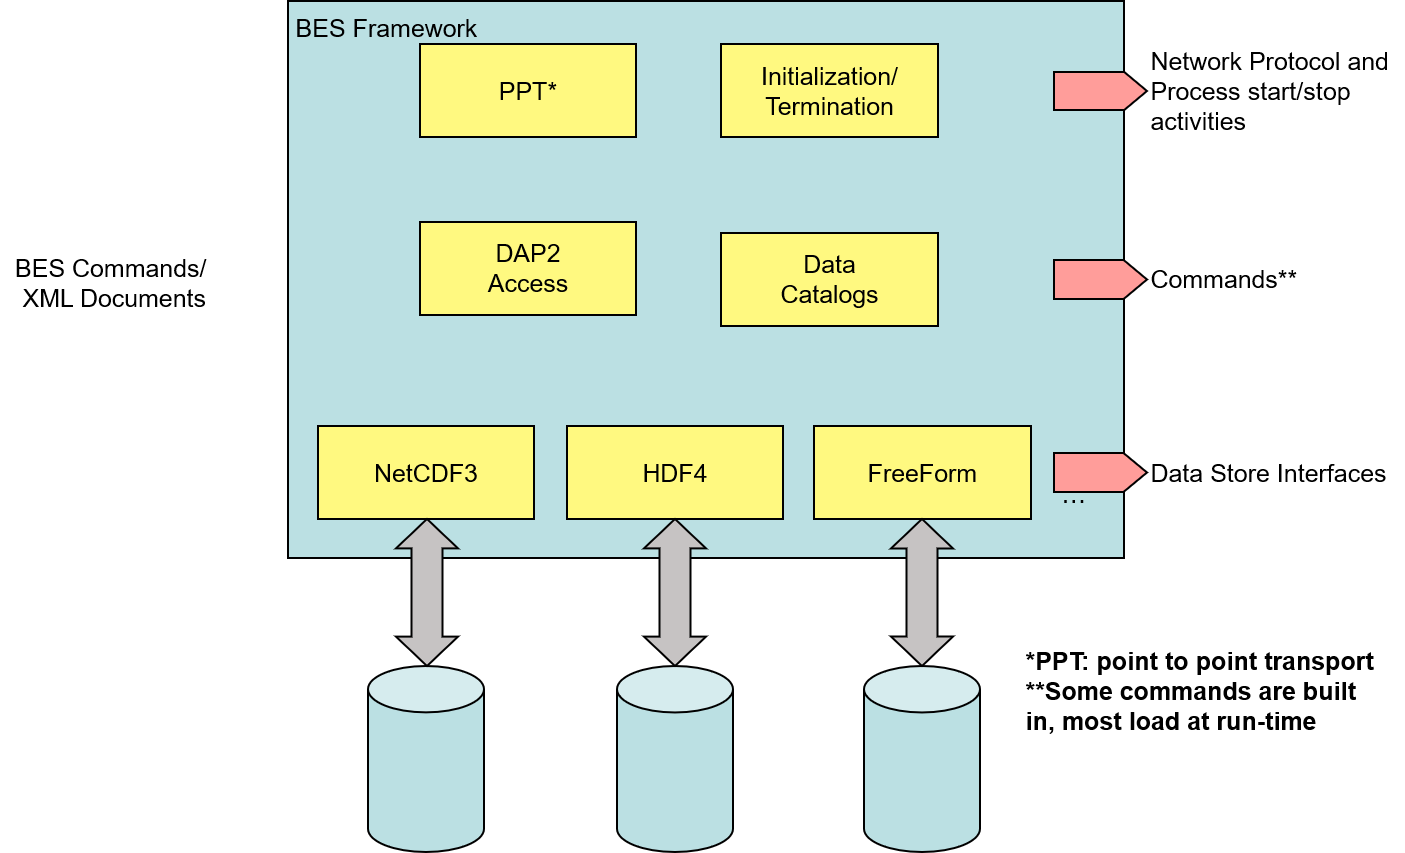
\includegraphics[width=4in,scale=1.0]{BES.png}
    \caption{BES Framework}
    \label{fig:BES}
\end{figure}
\subsubsection{BES}
\autoref{fig:BES} shows the general representation for the BES server within the standard Hyrax server. \cite{HyraxArchitecture} From this figure there is a hierarchy to the process of the BES. The first is the Network Protocols with the examples of PPT and Initialization/Termination, these are not the only options but are not something developers will likely need to deal with. The second is the BES commands which define how data is to be manipulated and handled. The third and final level is the interface which connects the BES to the data servers that house the data. For the sake of NASA JPL this will be their data servers, see a later section for information on their data types. The focus of the project will be on the BES command and the pull from the source, with more focus on commands. The commands will take the data returned from the server and translate it into the CovJSON standard. \autoref{fig:jsonstringarray} is an example of this which can already be found in the BES file, “FoDapJsonTransform.cc,” which transforms a DAP object into JSON. \cite{FoDapJsonTransform}
To go into too much detail this function takes in the return information from a call and turns it into a JSON Object. The code being developed from CovJSON will be similar to this example, although its base system will be from pycovjson rather than just this file. 
\subsubsection{Conclusion}
The functionality of the Hyrax server is instrumental for this project as most, if not all, components will have to eventually be implemented within it. While most coding of the project is dedicated to the BES, it is mandatory for developers to be able to understand and work with all pieces of Hyrax in order to make a complete and functional project.
\begin{figure}[H]
    \centering
    \lstinputlisting[language=XML]{olsf_config.xml}
    \caption{Initial setup for generic OLFS}
    \label{fig:OLFS}
\end{figure}

\begin{figure}[H]
    \centering
2    \lstinputlisting[language=C++]{json_string_array.cc}
    \caption{Function for translating scientific data formats into JSON}
    \label{fig:jsonstringarray}
\end{figure}
\subsection{Component: Data Access Protocol}
\subsubsection{Purpose}
The Data Access Protocol (DAP) is a protocol for accessing highly structured metadata and data organized as name-datatype-value tuples. OPeNDAP is well suited for allowing a client computer access to scientific data stored on a server computer that is networked with the client computer. The OPeNDAP protocol is one of the primary components of the project, as the team will be implementing a CovJSON data response handler module for the protocol. 
\subsubsection{Viewpoint}
OPeNDAP has a number of different data response handlers previously built into it, and the design of the project's CovJSON response handler will follow the same design as these previously built handlers. Therefore, the dependency design viewpoint makes the most sense as it will be a part of an integrated system. \cite{IEEE}
\subsubsection{Concerns}
The major concern regarding the data access protocol is that the CovJSON response handler will need to be adequately test and debugged before it can be fully integrated into the OPeNDAP project. As always, time is a concerning factor, and it will be imperative for the developers to utilize project resources effectively to remain on schedule.
\subsubsection{Functionality}
The OPeNDAP CovJSON response handler will define a C++ based API that Hyrax's BES service will use to retrieve coverage data from a database. The response handler functionally defines the data types, data structures, objects, and function prototypes necessary for BES to convert and transmit requested data back to the client from the Hyrax server. Fundamental protocol functionality includes transmission of data, conversion of data, and receiving of data. \autoref{fig:opendapflow} shows the data request/retrieval flow for OPeNDAP; OPeNDAP provides the BES an interface that it can use to request and move scientifically formatted data from a database. All of this functionality already exists within the currently implemented scientific data handlers in OPeNDAP, therefore, the design of the DAP/BES interface and functions will rely heavily upon previously designed implementations to avoid having to reinvent the wheel, so to speak.
\begin{figure}[H]
    \centering
    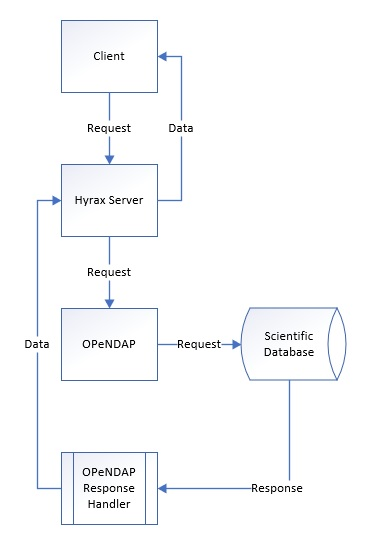
\includegraphics[width=3in,scale=0.75]{OPeNDAP_flow_chart.jpg}
    \caption{OPeNDAP Flow Chart}
    \label{fig:opendapflow}
\end{figure}
\subsection{Component: Data Format}
\subsubsection{Purpose}
The purpose of adding CoverageJSON to the available data formats in OPeNDAP is to accommodate web development needs based on the data held in OPeNDAP. CoverageJSON allows for richer application development due to it being an extension of JSON language, which is tailored for conveying data distinguished by its space-time coordinates. JSON is one of the more common standards for retrieving data from a source and makes CoverageJSON a popular choice for those unfamiliar with scientific data formats.   

\subsubsection{Viewpoint}
The view point for this component is information due to it being directly related and composed of the information handling and formatting portions of the project. \cite{IEEE}

\subsubsection{Concerns}
The primary concern regarding the data format is the possibility of an incorrect CoverageJSON encoding, since the requirement calls for multiple different data types to be changed into CoverageJSON this may present a problem in conversion methods. This will also require more knowledge of BES commands and managing the data correctly. 

\subsubsection{Functionality}
A sample of the CoverageJSON format is shown in \autoref{fig:covjson}. Since CovJSON is based on JSON, the data is broken down into categories, i.e. type, and domain. Those categories can have subcategories associated with them as a means of relying more data at once. JSON is notable in its ability to be human read, allowing developers to more easily manage the data that they receive.
\begin{figure}[H]
    \centering
    \lstinputlisting[language=XML]{covjson.xml}
    \caption{CoverageJSON Example}
    \label{fig:covjson}
\end{figure}
The implementation of CoverageJSON into OPeNDAP will be heavily based off of the current JSON handling in OPeNDAP. The actual logic behind the conversion from other scientific formats into CoverageJSON will be based off of the PyCovJSON python program developed by NASA JPL, which is able to view and perform conversions into CoverageJSON from common scientific data formats. The scientific data formats primary function is to structure and organize the metadata and data for a given format. Design of the response handler will conform to CovJSON language definitions and structure. 

\subsection{Component: Testing}
\subsubsection{Purpose}
The purpose of having predefined testing designs laid out is to create our implementation with testability in mind during the development process. This project will also have tests created during the implementation itself to minimize the overall level of effort exerted in testing. Functionality is inherently easier to test when it is fresh on the developer’s mind, so testing close to the time of implementation will be the goal.

\subsubsection{Viewpoint}
The viewpoint of testing will be interaction. Interaction defines, "strategies for interaction among entities, regarding why, where, how, and at what level actions occur." \cite{IEEE} The testing that will occur is to ensure correctness among the CovJSON handler and the hyrax server elements.

\subsubsection{Concerns}
The primary concern for unit testing is ensuring that the quality of tests created is high and that they accurately test the functionality of the implementation. Inadequate testing could lead to problems not being located and issues arising in the future development of the project; the goal will be to catch all errors as soon as possible so that they cannot inhibit further development.

\subsubsection{Functionality}
The testing that will occur on the implementation will be done through unit tests in the \gls{CppUnit} testing framework for C++ code. The unit testing will be done with the goal of having 90 percent code coverage when the implementation and testing are complete. The code coverage percentage goal may change due to feedback from the OPeNDAP team, as one of the primary goals in ensuring testing on the implementation is to allow it to be pulled into the OPeNDAP source code. The purpose of using the Cppunit framework is to align the work we do with the work that the OPeNDAP team does. Having consistent frameworks makes it easier for a hand off to occur between the developers and OPeNDAP.

\autoref{fig:cppunit} is an example code snippet of a CppUnit unit test. A short rundown of the code and explanation of the usefulness of testing frameworks will now be given. In this given example two values of money are created, and another is added to one of those constants. These values are now compared with CPPUNIT\_ASSERT which will either be true or false. If an assertion fails, or is not true, then the program will throw an error. The benefit of having a testing framework allows for quick and easy writing of unit tests to those who know the framework. \\This project will likely require manual and randomly created tests to ensure the safety of the code, this is simply because this is to become production code. The usefulness of the random tests is yet to be seen in this project, but will allow for testing beyond the scope of what can be thought of by the developers. However random tests may not be a requirement of OPeNDAP, and this section will be changed to reflect that later.   

\begin{figure}[h]
    \centering
	\lstinputlisting[language=C++]{CppUnit.cpp}
    \caption{CppUnit Example}
    \label{fig:cppunit}
\end{figure}

\subsection{Component: User Interface}
\subsubsection{Purpose}
The purpose of the user interface portion of this project is to allow users to be able to select data format types they need from the NASA JPL servers. This will include being able to have their data in the CoverageJSON format, which will be the addition made to the already implemented Hyrax user interface. 

\subsubsection{Concerns}
The primary concern for the user interface implementation is ensuring usability while adding the functionality to make a request for CoverageJSON format. Adding in the new functionality may cause conflicts from an interface standpoint, as it may interfere with the current interface elements.

\subsubsection{Viewpoint}
The view point for this component is logical since it is a system that is already in place and our project just entails making modifications to the current interface implementation. \cite{IEEE}

\subsubsection{Functionality}
The user interface development portion of this project will involve making modifications to the current implemented interface. The current plan for the modification will be the addition of another button on the OPeNDAP server dataset access form which is shown in \autoref{fig:opendapui}. This modification may change through feedback from the OPeNDAP team, or the modification to the UI may not happen at all, as it will also be possible to request data in the CoverageJSON format through a corresponding data url, which is currently how JSON formatting is requested.

\autoref{fig:opendapui} is a screen shot of the current data selection UI implemented in OPeNDAP. While it may seem bland to some, the purpose of the UI is to enable data scientists to get information that they need quickly. 

\begin{figure}[H]
    \centering
    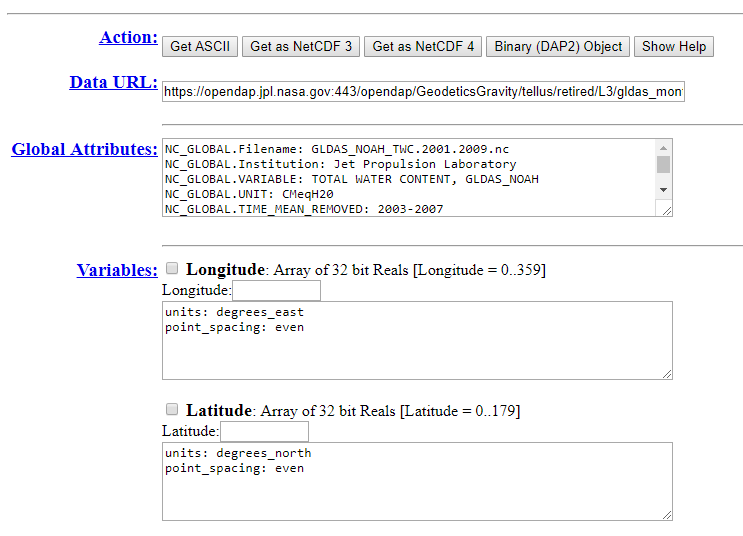
\includegraphics[width=5in,scale=1.0]{opendapui.PNG}
    \caption{OPeNDAP Server Dataset Access Form}
    \label{fig:opendapui}
\end{figure}
\subsubsection{Conclusion}
This section may be a little light, but this is due to the fact that this project is not targeted at the creation of a user interface. However, adding to the current implementation of the user interface is requirement of this project, it just does not entail much change by the development team. As stated previously, if this were to become a requirement or became a higher priority by the team then this section will change to accommodate those new requirements. 

\newpage
\section{Glossary}
\printglossary[style=mylong]

\newpage
\nocite{*}
\bibliographystyle{IEEEtran}
\bibliography{references}

\end{document}